\documentclass[11pt]{article}
\usepackage[margin=1in]{geometry}
\usepackage[T1]{fontenc}
\usepackage{lmodern}
\usepackage{amsmath,amssymb}
\usepackage{graphicx}
\usepackage{booktabs}
\usepackage{tabularx}
\usepackage{enumitem}
\usepackage{caption}
\usepackage[hidelinks]{hyperref}
\setlist{itemsep=2pt,topsep=4pt}

\title{Do Perturbation Models Compose Under Their Own Output?\\[4pt]
\large Midterm Report --- GenAI in Biomedicine, CMU, Fall 2026}
\author{Shreyan Nalwad (\texttt{snalwad}) \and Sri Datta Bandreddi (\texttt{sbandred})}
\date{November 6, 2026}

\newcommand{\pd}{Pearson~$\delta$}

\begin{document}
\maketitle

\begin{abstract}
Perturbation models predict a cell's expression after a genetic perturbation, and their
output lives in the same space as their input. We ask whether feeding a prediction back in,
$f(f(x, A), B)$, reproduces the measured double perturbation $A{+}B$, which a virtual-cell
``world model'' would require. On Norman et al.\ (2019), with all singles in training and
all 131 doubles held out, the additive baseline (control + effect of $A$ + effect of $B$)
reaches \pd{} 0.873. GEARS, trained only on singles, reaches 0.673 and has more than twice
the additive error on the top-20 genes (0.181 vs.\ 0.082). A split-half design shows that
non-additivity is a reproducible property of each pair (Spearman 0.94 across disjoint
cells), and additive error rises fivefold from the least to the most non-additive tertile.
Finally, GEARS's predicted shift does not depend on its input cell, so its rollout is
additive by construction; scGPT is the model where composition remains an open question.
\end{abstract}

%-------------------------------------------------------------------------
\section{Introduction}

Perturbation response models such as GEARS~\cite{gears}, scGPT~\cite{scgpt} and
State~\cite{state} predict how a cell's expression changes after a genetic perturbation. A
control cell goes in; a predicted perturbed profile comes out. Because input and output
share one expression space, a prediction can in principle be fed back in and perturbed
again: $\mathrm{predict}(\mathrm{predict}(x, A), B)$.

If a model has learned a reusable representation of cell state, that rollout should
approximate the measured double perturbation $A{+}B$. If it is only a one-step map from
control cells, it should not. As far as we know, no published work has tested which is the
case.

The question matters because of where the field is heading. Proposals for virtual-cell
world models~\cite{xingsong} envision simulating cells under sequences of interventions.
That needs a model whose output is a valid input. We do not build such a model; we test
whether current models meet this precondition on the one dataset where it can be checked
against measured combinations.

The starting point is sobering. Ahlmann-Eltze \& Huber~\cite{ahlmann} showed that on Norman
et al.'s~\cite{norman} doubles, deep models do not beat simple addition of the two single
effects. They evaluated only the joint prediction. We ask the complementary question: do
models compose under their own output? Our test trains on single perturbations only, holds
out every double, and compares three predictions per pair: the model's joint prediction of
$A{+}B$, its sequential rollout $A$ then $B$, and simple baselines, mainly addition.

\paragraph{Changes since the proposal, in response to reviewers.}
\begin{enumerate}
  \item \textbf{Two rollout arms (point 1).} Norman's doubles keep guide $A$ active
  throughout, which neither rollout reproduces exactly. We report both \emph{carried} (the
  second step gets label $B$ only) and \emph{restated} (it gets $A{+}B$).
  \item \textbf{Round-trip gate (point 2).} No model enters the comparison until it passes a
  full input $\to$ output $\to$ input check on real and generated inputs.
  \item \textbf{Split-half cells (point 3).} Each condition's cells are split into two
  random halves: one only for measuring non-additivity, the other for everything else.
  \item \textbf{Two GEARS training regimes (point 4).} GEARS is trained on its own standard
  split as a diagnostic and on our strict singles-only split for the experiment.
\end{enumerate}
We also narrowed scope to fit a 4.5-week calendar. The ComboSciPlex and Replogle experiment
is cut. Geneformer is excluded because it outputs an embedding shift with no expression
decoder. State and CPA are out for time.

%-------------------------------------------------------------------------
\section{Related Work}

The closest prior work shows that simple addition beats deep models on Norman doubles; ours
differs by testing rollout, using a singles-only split, and controlling for measurement
noise.

\paragraph{Predicting doubles from singles.} Norman et al.~\cite{norman} measured 131
pairwise CRISPRa perturbations and all their singles in K562 cells. Most pairs combine
roughly additively, with a minority showing synergy, buffering or new behaviour. The
dataset is the standard benchmark for combinatorial prediction.

\paragraph{Deep perturbation models.} GEARS~\cite{gears} encodes each perturbed gene
through a gene-ontology graph and predicts the perturbed expression of a control cell.
scGPT~\cite{scgpt} fine-tunes a pretrained transformer for the same task.
CPA~\cite{cpa} and scGen~\cite{scgen} represent perturbations as vectors in a learned
latent space. State~\cite{state} is a recent large transition model. All are trained and
evaluated as one-step maps, control $\to$ perturbed.

\paragraph{Simple baselines beat deep models.} Ahlmann-Eltze \& Huber~\cite{ahlmann} showed
that adding the two single shifts beats GEARS, scGPT and other foundation models on Norman
doubles. Related benchmarks~\cite{perteval,csendes,systema} found that much apparent
accuracy comes from shifts shared by all perturbations. Table~\ref{tab:diff} summarises how
our study differs.

\begin{table}[h]
\centering
\caption{How this work differs from prior benchmarks.}
\label{tab:diff}
\begin{tabularx}{\linewidth}{lXX}
\toprule
 & Prior benchmarks & This work \\
\midrule
What is scored & Joint prediction $f(x, A{+}B)$ only & Joint and rollout $f(f(x, A), B)$, both arms \\
Training split & GEARS default; some doubles in training & All singles train, all 131 doubles test \\
Noise control & Strata and scores from the same cells & Strata from cell half 1, scores from half 2 \\
\bottomrule
\end{tabularx}
\end{table}

\paragraph{Latent-space composition.} scGen and CPA add perturbation vectors inside a
latent space, the closest prior idea to rollout. There, composition is an assumption built
into the architecture, not a property tested on measured doubles. It also happens in latent
space rather than by re-entering the model through its expression input.

\paragraph{Virtual cells and world models.} Xing \& Song~\cite{xingsong} argue for virtual
cells that can be rolled forward under sequences of interventions. Such a model needs its
outputs to be valid inputs, which is the precondition we test.

%-------------------------------------------------------------------------
\section{Methodology}

We train on single perturbations only, score every held-out double on cells never used to
select it, and compare models with the additive baseline pair by pair.

\paragraph{Research questions.}
\begin{itemize}
  \item \textbf{RQ1, joint.} Trained on singles only, does a model predict held-out doubles
  better than addition, and is any advantage concentrated in measurably non-additive pairs?
  \item \textbf{RQ2, composition.} Does the rollout $f(f(x, A), B)$ approach the measured
  double as well as the joint prediction?
  \item \textbf{RQ3, diagnosis.} When rollout fails, is it because the model cannot accept
  non-control input, or because its own predictions drift away from real cells?
\end{itemize}

\paragraph{Data.} Norman et al.~\cite{norman} CRISPRa Perturb-seq in K562 cells,
GEARS-processed: 91,205 cells $\times$ 5,045 genes, 105 singles and 131 doubles. Every
double has both of its singles measured.

\paragraph{Strict split.} All singles and control are training conditions; all 131 doubles
are test. GEARS's default split instead trains on some doubles. Under ours, a model and the
additive baseline see the same information. For GEARS, 10\% of the singles not involved in
any double are held out for validation.

\paragraph{Split-half design.} Each condition's cells are split at random into two halves,
repeated over 5 seeds. Half 1 is used for measurement only: the non-additivity score
$\eta$, and the top-20 differentially expressed genes (DEGs) used for scoring. Half 2 is used
for everything else: inputs to baselines and models, and the targets they are scored
against. The noise that puts a pair in a ``highly non-additive'' group therefore never
appears in its scoring target. With $\Delta$ the pseudobulk shift from control in half $h$,
\begin{equation}
r_h = \Delta_{AB} - \Delta_A - \Delta_B, \qquad \eta_h = \lVert r_h \rVert .
\end{equation}
Because the halves have independent noise, $r_1 \cdot r_2$ is an unbiased estimate of the
true squared residual, which tells us how much of $\eta$ is signal. Pairs are grouped into
$\eta$ tertiles using half 1.

\paragraph{Baselines.} All are built from half-2 pseudobulks of training conditions
(Table~\ref{tab:nulls}). Low-rank additive is the singles-only analogue of
Ahlmann-Eltze \& Huber's linear baseline.

\begin{table}[h]
\centering
\caption{Baselines and their prediction for $A{+}B$.}
\label{tab:nulls}
\begin{tabular}{ll}
\toprule
Baseline & Prediction \\
\midrule
No change & control \\
Train mean & control + average single shift \\
Additive & control + $\Delta_A + \Delta_B$ \\
Low-rank additive & control + rank-10 SVD-denoised $\Delta_A + \Delta_B$ \\
\bottomrule
\end{tabular}
\end{table}

\paragraph{Models.} Each model sits behind one interface, $\mathrm{predict}(X,
\mathrm{pert}) \to X$, which takes cells and returns cells in the same gene space. GEARS's
own \texttt{predict()} samples control cells internally, so our adapter builds its input
graph from the expression we pass. Predictions are anchored to the pseudobulk of their
input condition, so models are not penalised for sampling noise in the $\sim$300 input
cells. For each held-out pair we compute:
\begin{itemize}
  \item \textbf{joint:} $f(x_0, \{A, B\})$
  \item \textbf{carried rollout:} $f(f(x_0, A), B)$
  \item \textbf{restated rollout:} $f(f(x_0, A), \{A, B\})$
  \item \textbf{measured-input rollout:} $f(x_A, B)$, starting from real $A$-perturbed
  cells, which separates a failure to compose from a failure on generated input (RQ3)
  \item \textbf{both orders,} $A$ then $B$ and $B$ then $A$
\end{itemize}
For GEARS on its standard split, doubles seen in training are excluded from scoring.

\paragraph{Round-trip gate.} Before joining the comparison, a model must pass a check on
singles. Real $A$-perturbed cells passed through with no new perturbation should come back
nearly unchanged ($r > 0.95$), and so should the model's own predicted $A$ state. Failure on
real input means composition cannot be tested for that model; failure only on generated
input means distribution shift.

\paragraph{Consistency checks.} Order dependence ($A\to B$ vs.\ $B\to A$) and saturation
(applying $A$ twice) are reported as computational checks only. Norman measures joint
perturbations and cannot validate either biologically.

\paragraph{Metrics and inference.} MSE on the top-20 DEGs, and Pearson correlation of
predicted vs.\ observed shift from control (\pd), over all genes and over the top-20 DEGs.
Per-pair results are averaged over the 5 seeds. All 95\% intervals come from 2,000
bootstrap resamples over pairs, never cells, because the pair is the unit of inference.

%-------------------------------------------------------------------------
\section{Experiments (Preliminary Results)}

Addition is the strongest predictor of held-out doubles, and GEARS trained on singles has
more than twice its error. Setup: 131 held-out doubles, 5 random half-splits, per-pair
results averaged over splits, 95\% bootstrap intervals over pairs. GEARS used seed 1 and 20
epochs for each regime.

\subsection{Baselines and GEARS joint prediction}

Addition wins on every metric (Table~\ref{tab:main}, Figure~\ref{fig:hier}). Denoising the
singles makes it worse: low-rank addition beats plain addition on only 23 of 131 pairs.

\begin{table}[h]
\centering
\caption{Held-out doubles, mean [95\% CI]. Lower MSE and higher \pd{} are better.
No-change predicts zero shift, so its correlation is undefined.}
\label{tab:main}
\small
\begin{tabular}{lrccc}
\toprule
Predictor & Pairs & MSE, top-20 DEGs & \pd, all genes & \pd, top-20 DEGs \\
\midrule
\textbf{Additive} & 131 & \textbf{0.081} [0.067, 0.096] & \textbf{0.873} [0.857, 0.886] & \textbf{0.959} [0.952, 0.964] \\
Low-rank additive & 131 & 0.140 [0.123, 0.158] & 0.789 [0.766, 0.810] & 0.870 [0.847, 0.891] \\
GEARS, strict split & 128 & 0.181 [0.161, 0.204] & 0.673 [0.645, 0.700] & 0.862 [0.833, 0.888] \\
GEARS, standard split & 71 & 0.232 [0.194, 0.271] & 0.605 [0.558, 0.653] & 0.798 [0.740, 0.851] \\
Train mean & 131 & 0.575 [0.494, 0.656] & 0.533 [0.488, 0.575] & 0.644 [0.582, 0.700] \\
No change & 131 & 0.734 [0.643, 0.824] & undefined & undefined \\
\bottomrule
\end{tabular}
\end{table}

\begin{figure}[h]
\centering
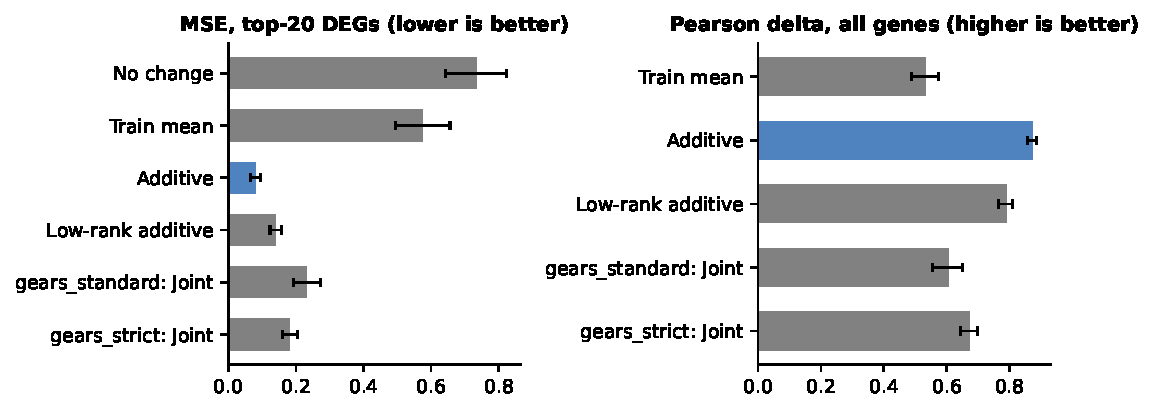
\includegraphics[width=\linewidth]{../figures/fig2_null_hierarchy.pdf}
\caption{Baselines and GEARS joint prediction on held-out doubles, with 95\% bootstrap
intervals over pairs.}
\label{fig:hier}
\end{figure}

GEARS is scored on fewer pairs for two reasons. Three doubles contain a gene outside GEARS's
gene-ontology graph (IER5L+LYL1, RHOXF2BB+SET, RHOXF2BB+ZBTB25). On its standard split,
GEARS also trains on 57 doubles, which are excluded. On the same pairs, addition scores
0.082 (128 pairs) and 0.085 (71 pairs), so the gap is not a pair-set artefact.

On the strict split, GEARS's MSE exceeds addition's by 0.100 [0.077, 0.122], and GEARS is
better on only 14\% of pairs. On the standard split the gap is 0.148 [0.106, 0.187], with
GEARS better on 13\%. GEARS beats only the train-mean and no-change baselines. The two GEARS
rows are not directly comparable, because the standard set includes pairs with a single
never seen in training.

\subsection{Non-additivity is a reproducible property of each pair}

$\eta$ measured on two disjoint cell halves agrees with Spearman 0.944 (per seed 0.932 to
0.955; Figure~\ref{fig:eta}). The cross-half estimate of true $\eta^2$ is positive for
99.5\% of pairs and accounts for 61\% of measured $\eta^2$. $\eta$ is therefore mostly
signal, with a noise share of about 40\%.

\begin{figure}[h]
\centering
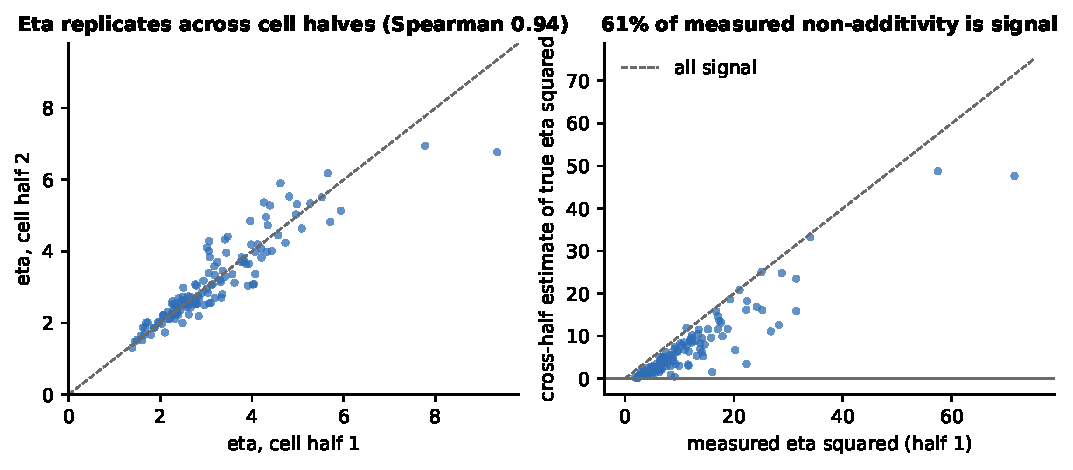
\includegraphics[width=\linewidth]{../figures/fig1_eta_reliability.pdf}
\caption{Left: $\eta$ measured on two disjoint cell halves. Right: the cross-half estimate
of true $\eta^2$ against measured $\eta^2$; the dashed line is ``all signal''.}
\label{fig:eta}
\end{figure}

\subsection{Additive error rises with non-additivity}

With $\eta$ taken from half 1 and error from half 2, $\eta$ and additive MSE correlate with
Spearman 0.82 across pairs (Figure~\ref{fig:addeta}). Additive error rises about fivefold
from the low to the high tertile; GEARS stays above it throughout, and the gap narrows only
where interactions are strongest (Table~\ref{tab:tert}). The most non-additive pairs are
dominated by the CEBP family (CEBPA+CEBPB, CEBPA+CEBPE, CEBPE+SET, CEBPA+KLF1), consistent
with the redundant differentiation programmes Norman et al.\ described.

\begin{figure}[h]
\centering
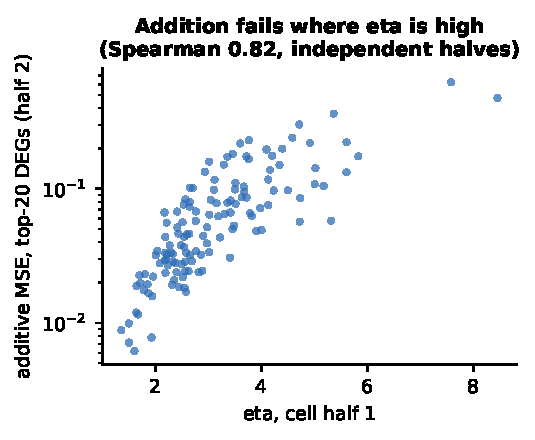
\includegraphics[width=0.55\linewidth]{../figures/fig3_additive_vs_eta.pdf}
\caption{Additive error (half 2) against $\eta$ (half 1), one point per held-out double.}
\label{fig:addeta}
\end{figure}

\begin{table}[h]
\centering
\caption{MSE on the top-20 DEGs by $\eta$ tertile, strict split, same 128 doubles.}
\label{tab:tert}
\begin{tabular}{lcc}
\toprule
$\eta$ tertile & Additive & GEARS, strict \\
\midrule
Low & 0.028 & 0.140 \\
Mid & 0.064 & 0.210 \\
High & 0.153 & 0.194 \\
\bottomrule
\end{tabular}
\end{table}

\subsection{Round-trip gate}

Strict GEARS passes on the 5 singles with the most cells (KLF1, BAK1, CEBPE, ETS2,
UBASH3B). Real $A$-perturbed cells passed through with no new perturbation come back with
$r = 0.999$ on expression and 0.80 to 0.99 on shifts from control. Its own predicted states
behave the same.

The pass is structural, not learned. Applying $A$ twice moves the cell exactly as far as
applying it once (saturation ratio 1.0 for all five genes). The GEARS source explains why:
input expression enters only as a final residual, $\mathrm{out} = x + g(\mathrm{pert})$, and
$g$ ignores the input cell. GEARS's prediction is therefore independent of the state it
starts from.

%-------------------------------------------------------------------------
\section{Analysis and Ablations}

The midterm results already answer RQ1 for GEARS (it does not beat addition) and reduce RQ2
for GEARS to a comparison of two additive constructions.

\paragraph{$\eta$ is a sound way to group pairs.} The worry was that ``highly non-additive''
pairs might just be the noisiest ones, making their high error a regression-to-the-mean
artefact. The split-half design rules this out: $\eta$ replicates across disjoint cells
(Spearman 0.94), and every error is scored on the half not used to define the groups. The
high-$\eta$ tertile is where a model with real interaction knowledge has room to beat
addition.

\paragraph{Addition is a hard bar, and the room above it is concentrated.} Most of
addition's error sits in the top $\eta$ tertile, five times the low tertile's. An overall
average therefore mostly reflects easy, near-additive pairs. The rollout analysis after the
midterm is planned as advantage over addition as a function of $\eta$, not as one average.

\paragraph{Ablation: smoothing the singles does not help.} Low-rank addition is worse than plain
addition on 82\% of pairs. With pseudobulks from roughly 100 to 300 cells, the single
effects are already precise, so the rank-10 projection removes more real signal than noise.
A singles-only model must know something about how effects interact to beat addition.

\paragraph{GEARS has not learned interactions, and it cannot carry state.} On the strict
split, GEARS's error exceeds addition's in every tertile. Its gap narrows in the high
tertile (0.194 vs.\ 0.153) but does not reverse. Its predicted shift also ignores the input
cell, so its rollouts are fixed by construction:
\begin{equation}
\text{carried: } x + g(A) + g(B), \qquad \text{restated: } x + g(A) + g(A,B).
\end{equation}
Order cannot matter, and applying $A$ twice simply doubles its shift. For GEARS, the
remaining empirical question is whether its own singles, $g(A) + g(B)$, land closer to the
measured double than its joint $g(A,B)$. scGPT, whose output does depend on the input, is
where composition is a genuinely open question.

\paragraph{Caveat: $\eta$ partly tracks effect size.} $\eta$ correlates with the size of the
double's shift (Spearman 0.54), and shift size alone predicts additive error about as well
(0.58). $\eta$ relative to the shift barely predicts it (0.15), and the scale-free \pd{}
hardly falls across tertiles (0.880 to 0.862). Part of the trend is ``bigger perturbations
have bigger absolute errors''. For the final report we will compare models with addition
within tertiles, which cancels scale, and check conclusions with relative $\eta$ or effect
size as a covariate.

%-------------------------------------------------------------------------
\section{Limitations}

The midterm results rest on one dataset, one GEARS seed and joint predictions only.
\begin{itemize}
  \item \textbf{One dataset.} Norman is the only public set with doubles and all their
  singles, so we cannot test generality on another cell type or perturbation modality.
  \item \textbf{Biology of rollout.} Norman's guides act together for the whole experiment.
  Neither rollout arm matches that exactly, and order and saturation cannot be validated
  biologically.
  \item \textbf{One GEARS run.} Each regime was trained once (seed 1, 20 epochs, default
  hyperparameters). Seed-to-seed variation and tuning are untested.
  \item \textbf{Unpredictable pairs.} GEARS cannot perturb RHOXF2BB, KIAA1804 or IER5L, so 3
  of 131 doubles are missing from its scores.
  \item \textbf{Effect-size confound.} $\eta$ partly measures the size of the perturbation,
  not only its non-additivity (Section 5).
  \item \textbf{Rollout not yet run.} The midterm reports joint predictions only; the
  composition results are still to come.
\end{itemize}

%-------------------------------------------------------------------------
\section{Timeline for Remaining Work}

The full rollout experiment runs next; by November 15 we decide whether scGPT passes the
round-trip gate or the study proceeds with GEARS alone.

\begin{table}[h]
\centering
\caption{Remaining milestones.}
\begin{tabular}{ll}
\toprule
Date & Milestone \\
\midrule
Nov 6 & Midterm report (this document) \\
Nov 15 & Decide: keep scGPT, or GEARS only \\
Nov 22 & Final-report figures drafted \\
Dec 3 & Final report and presentation \\
\bottomrule
\end{tabular}
\end{table}

\paragraph{Before the November 15 decision.}
\begin{enumerate}
  \item Full rollout on strict GEARS: both arms, both orders, and the measured-input control (Shreyan).
  \item Standard-split GEARS rollout as the diagnostic comparison (Shreyan).
  \item scGPT adapter, then the round-trip gate; joint and rollout only if it passes (Shreyan).
  \item Rollout analysis: advantage over addition vs.\ $\eta$ with slope and CI, order dependence vs.\ $\eta$, arm comparison (Datta).
\end{enumerate}

\paragraph{After it.}
\begin{enumerate}
  \item Stability: saturation ratio and drift from real cells over 1 to 10 steps (Datta).
  \item Effect-size checks from Section 5: within-tertile comparisons and relative $\eta$ (Datta).
  \item Draft final-report figures by November 22; final report and presentation by December 3 (both).
\end{enumerate}

\paragraph{Cut order if time runs short:} the discriminator-based drift metric, then five
split seeds down to three, then scGPT, then the stability experiment.

%-------------------------------------------------------------------------
% Entries marked (verify) were written from memory; check venue and year before submission.
\begin{thebibliography}{99}
\bibitem{norman} T.~M. Norman et al. Exploring genetic interaction manifolds constructed from rich single-cell phenotypes. \emph{Science}, 2019. \url{https://doi.org/10.1126/science.aax4438}
\bibitem{ahlmann} C.~Ahlmann-Eltze and W.~Huber. Deep learning-based predictions of gene perturbation effects do not yet outperform simple linear baselines. \emph{Nature Methods}, 2025. \url{https://doi.org/10.1038/s41592-025-02772-6}
\bibitem{gears} Y.~Roohani, K.~Huang, and J.~Leskovec. Predicting transcriptional outcomes of novel multigene perturbations with GEARS. \emph{Nature Biotechnology}, 2024. \url{https://doi.org/10.1038/s41587-023-01905-6}
\bibitem{scgpt} H.~Cui et al. scGPT: toward building a foundation model for single-cell multi-omics using generative AI. \emph{Nature Methods}, 2024. \url{https://doi.org/10.1038/s41592-024-02201-0}
\bibitem{xingsong} Xing and Song. Virtual cell world model. \emph{Cell}, 2026. % (verify title)
\bibitem{cpa} M.~Lotfollahi et al. Predicting cellular responses to complex perturbations in high-throughput screens. \emph{Molecular Systems Biology}, 2023. % (verify)
\bibitem{scgen} M.~Lotfollahi, F.~A. Wolf, and F.~J. Theis. scGen predicts single-cell perturbation responses. \emph{Nature Methods}, 2019. % (verify)
\bibitem{state} Arc Institute. State: a transition model for cellular perturbation response, 2025. % (verify)
\bibitem{perteval} A.~Wenteler et al. PertEval-scFM: benchmarking single-cell foundation models for perturbation effect prediction. % (verify)
\bibitem{csendes} G.~Csendes et al. Benchmarking foundation cell models for post-perturbation RNA-seq prediction. % (verify)
\bibitem{systema} R.~Vi\~nas Torn\'e et al. Systema: systematic variation in perturbation response prediction. % (verify)
\end{thebibliography}

\end{document}
